\begin{explanationbox}
\textbf{\textcolor{CExplanation}{一句话直觉}}
两个量（正数或任意实数）之间的大小关系，其本质是“平方非负”这一简单事实的多种代数包装。

\medskip
\textbf{\textcolor{CExplanation}{核心拆解}}
\begin{description}[style=nextline, leftmargin=2.8em, labelsep=0.5em, itemsep=0.45em]
    \item[\textbf{要点一（平方差非负）：}] 最根本的来源是 $(a-b)^2 \ge 0$，展开即得 $a^2 + b^2 \ge 2ab$。
    \item[\textbf{要点二（均值转化）：}] 利用代换（如令 $x=\sqrt{a}, y=\sqrt{b}$）可将平方和形式转化为算术-几何平均形式。
    \item[\textbf{要点三（等价变形）：}] 各不等式可通过代数运算（如移项、平方、配方）互相推导，本质相同。
\end{description}

\medskip
\textbf{\textcolor{CExplanation}{几何本质（矩形与正方形）}}
以 $a+b \ge 2\sqrt{ab}$ 为例：周长固定的矩形中，正方形的面积最大。固定两边之和时，矩形面积最大与平方和最小均在两边相等时达到。

\medskip
\textbf{\textcolor{CExplanation}{代数意义（配方法）}}
不等式 $a^2 + b^2 \ge 2ab$ 等价于 $(a-b)^2 \ge 0$，这揭示了所有证明的起点：一个实数的平方非负。这是不等式证明最基础的配方法思想。

\medskip
\textbf{\textcolor{CExplanation}{考点价值（最值与证明）}}
\begin{itemize}[leftmargin=*, itemsep=0.5em, topsep=0.4em]
    \item \textbf{考法一（最值求解）：} 用于求解在给定约束（如和为定值、积为定值）下的最值（最大或最小）问题。
    \item \textbf{考法二（不等式证明）：} 作为证明链中的关键一步，用于放缩或建立不等关系，常见于综合证明题。
\end{itemize}

\medskip
\textbf{\textcolor{CExplanation}{顿悟点}}
\textbf{“一正二定三相等”}是使用基本不等式求最值的口诀，分别对应“正数条件”、“和或积为定值”、“等号成立条件”，这是确认常见定和、定积最值能否达到的检查方法；证明或放缩时不要求和或积为定值。

\medskip
\textbf{\textcolor{CExplanation}{使用场景}}
\begin{itemize}[leftmargin=*, itemsep=0.5em, topsep=0.4em]
    \item \textbf{场景一（直接套用）：} 题目中表达式明显符合 $x+y$ 与 $\sqrt{xy}$ 或 $x^2+y^2$ 与 $xy$ 的关系。
    \item \textbf{场景二（变形后使用）：} 通过常数代换、分母有理化、拆项、凑项等手段，将表达式化为可使用基本不等式的形式。
\end{itemize}

\medskip\textbf{统一的差值结构}
\[\frac{(a+b)^2}{4}-ab=\frac{(a-b)^2}{4},\qquad
 a^2+b^2-\frac{(a+b)^2}{2}=\frac{(a-b)^2}{2}.\]
当和固定时，差的绝对值越小，积越大、平方和越小；当正数积固定时，$(a+b)^2=4ab+(a-b)^2$，差的绝对值越小，和越小。
\begin{center}
\begin{tabular}{c|ccccc}
$a$&1&2&3&4&5\\ $b$&9&8&7&6&5\\ \hline
$ab$&9&16&21&24&25\\ $a^2+b^2$&82&68&58&52&50
\end{tabular}
\end{center}
积固定为16时，$(1,16),(2,8),(4,4)$ 的和依次为17、10、8。
\begin{center}
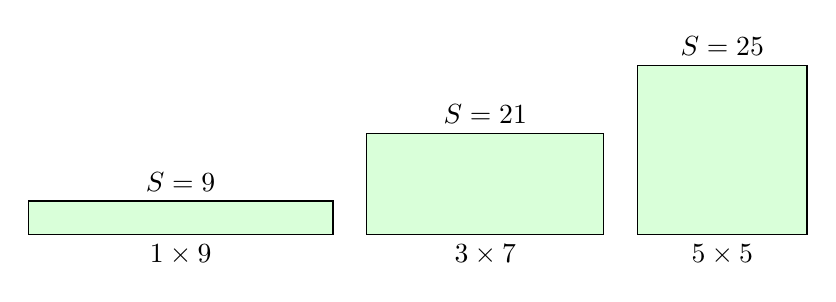
\begin{tikzpicture}[scale=.43]
\foreach \a/\b/\x in {1/9/0,3/7/10,5/5/18}{
\draw[fill=green!15] (\x,0) rectangle ++(\b,\a);
\node[below] at ({\x+\b/2},0) {$\a\times\b$};
\node[above] at ({\x+\b/2},\a) {$S=\pgfmathparse{int(\a*\b)}\pgfmathresult$};}
\end{tikzpicture}
\par 周长均为20，正方形面积最大。
\end{center}
\begin{center}
\begin{tikzpicture}[x=.65cm,y=.28cm]
\draw[->] (0,0)--(10,0) node[right]{$x$};
\draw[->] (0,0)--(0,19) node[above]{$y$};
\draw[green!50!black,thick,domain=.55:9.5,samples=100] plot (\x,{\x+9/\x});
\draw[dashed] (0,6) node[left]{$6$} -- (9.5,6);\draw[dashed] (3,0) node[below]{$3$}--(3,6);
\fill (3,6) circle (2pt) node[above right]{$(3,6)$};
\node at (7,16) {$y=x+9/x$};
\end{tikzpicture}
\end{center}

\end{explanationbox}
